\documentclass{article}
\usepackage{geometry}
\usepackage{graphicx}
\usepackage{amsmath}
\usepackage{amsfonts}
\usepackage{color}
\usepackage{listings}
\usepackage{float}
\geometry{a4paper,margin=1in}


\title{
\textbf{\begin{tabular}{c}Exercise 4: Real Time Continuous Media\end{tabular}}}
\author{\Large
\begin{tabular}{l@{\hspace{2em}}r}Zachary \textsc{Vogel}&  Priyanka \textsc{Pashte}\end{tabular}
\\[1.5ex]
\begin{tabular}{l@{\hspace{2em}}r}ECEN 5623 & Timothy \textsc{Scherr}\end{tabular}}
\date{March 5th, 2016}

\begin{document}
\lstset{language=C++,
                basicstyle=\ttfamily,
                keywordstyle=\color{blue}\ttfamily,
                stringstyle=\color{red}\ttfamily,
                commentstyle=\color{green}\ttfamily,
                morecomment=[l][\color{magenta}]{\#}
}
\maketitle

\section*{Problem 1}
\subsection*{USB hot-plug proof}
Here is the dmesg showing the uvc driver pulling up the device.
\begin{figure}[H]
    \centering
    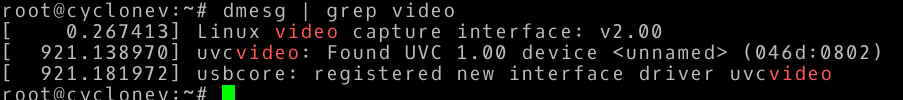
\includegraphics[width=0.8\textwidth]{dmesg.png}
    \caption{As you can see dmesg shows the uvc driver recognize that the camera was plugged in}
\end{figure}
\subsection*{UVC driver verify}
Here is a screenshot showing that we got the UVC driver installed on the DE1 board.
\begin{figure}[H]
    \centering
    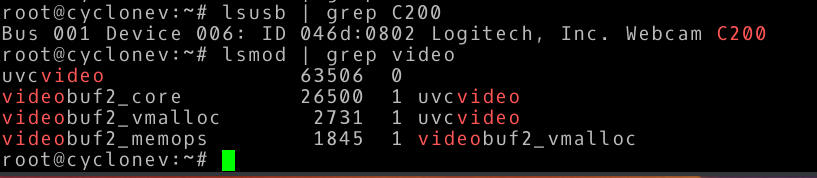
\includegraphics[width=0.8\textwidth]{lsmod_lsusb.png}
    \caption{As you can see the Logitech webcam appears as does the driver}
\end{figure}
\section*{Problem 2}
\subsection*{Use of tools such as camorama}
Here, we have taken a screenshot of camorama running and some settings being adjusted.
\begin{figure}[H]
    \centering
    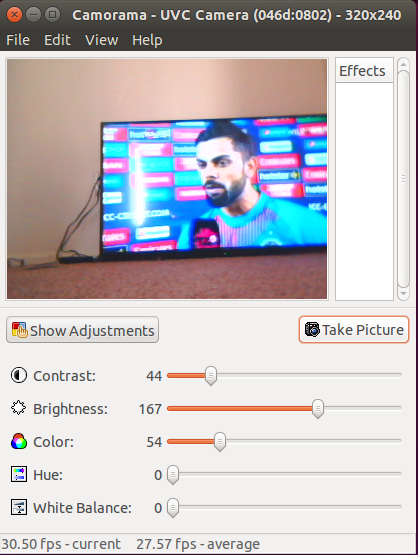
\includegraphics[width=0.6\textwidth]{Q2.png}
    \caption{The camorama application running with a captrued photo}
\end{figure}

\section*{Problem 3}
\subsection*{Build and Test}
We did install openCV on the DE1, but since we are using a laptop we should verify it is installed here. I used the official arch repositories for the installation.
\begin{figure}[H]
    \centering
    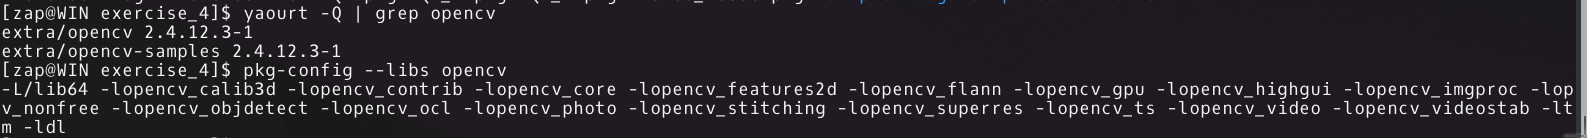
\includegraphics[width=\textwidth]{opencv_installed.png}
    \caption{Proof opencv is installed on the system}
\end{figure}
\subsection*{Streaming Verification}
Here, we have 2 examples of capture in progress.
\begin{figure}[H]
    \centering
    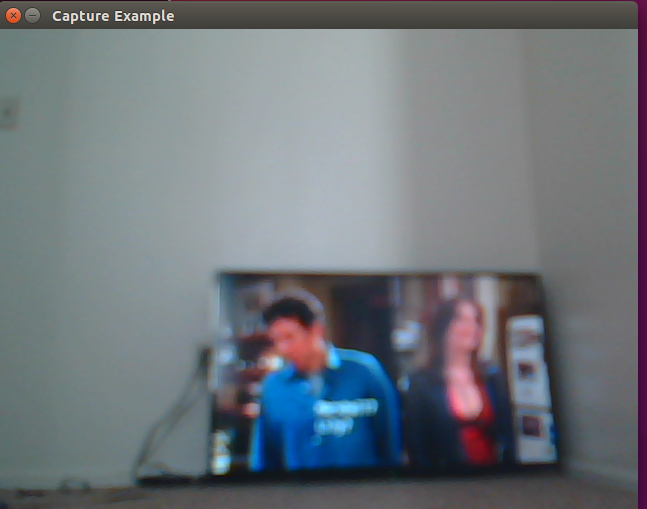
\includegraphics[width=0.8\textwidth]{Q3_1.png}
    \caption{An example of capture}
\end{figure}
\begin{figure}[H]
    \centering
    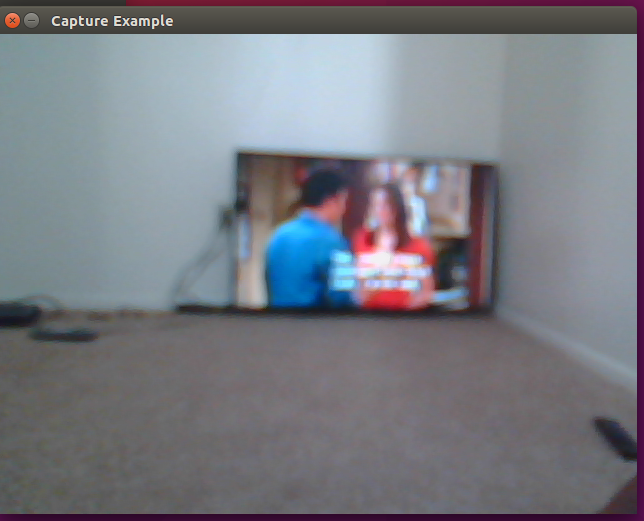
\includegraphics[width=0.8\textwidth]{Q3_2.png}
    \caption{An example of capture}
\end{figure}
\section*{Problem 4}
\subsection*{Demonstration of Tests}
Here we have a demonstration that we ran the canny transformation example code.
\begin{figure}[H]
    \centering
    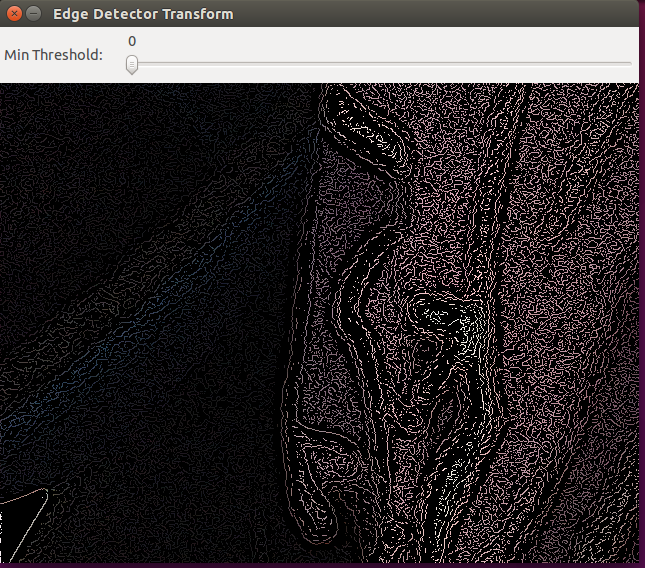
\includegraphics[width=0.6\textwidth]{Q4_1.png}
    \caption{An example of the canny transformation code running}
\end{figure}
\begin{figure}[H]
    \centering
    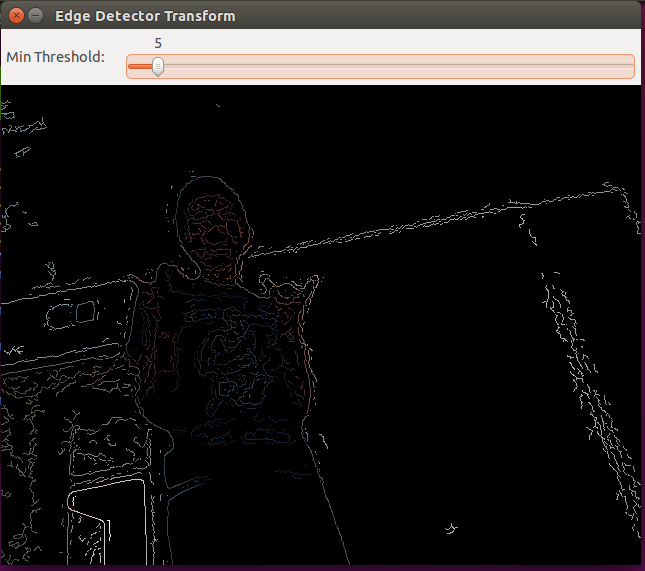
\includegraphics[width=0.6\textwidth]{Q4_2.png}
    \caption{An example of the same code, but using the slideruler for different results}
\end{figure}

\subsection*{Description of Tests}
The Canny Edge Detector is an edge detection operation that uses a multi-stage algorithm to detect a wide range of edges in images. It is the first derivative of a Gaussian and closely approximates the operator that optimizes the product of signal-to-noise ratio and localization. Canny Transform is known as the optimal detector and aims to satisfy three main criteria:
\begin{itemize}
	\item Low error rate: Meaning a good detection of only existent edges. 
	\item  Good localization: The distance between edge pixels detected and real edge pixels have to be minimized. 
	\item  Minimal response: Only one detector response per edge
\end{itemize}
\begin{lstlisting}
int lowThreshold=0; 
int const max_lowThreshold = 100; 
int kernel_size = 3;
int edgeThresh = 1; 
int ratio = 3;
\end{lstlisting}
First, we declare some variables. The variable ratio defines the lower:upper threshold as 3:1. The kernel size is set to  3. The initial value of the lower threshold is set to 0 and the maximum value that it can take is set to 100.
\begin{lstlisting}
vCapture* capture;
int dev=0; 
if(argc > 1)
{
    sscanf(argv[1], "%d", &dev);
    printf("using %s\n", argv[1]);
}
else if(argc == 1)
    printf("using default\n");
else
{
    printf("usage: capture [dev]\n");
    exit(-1);
}
\end{lstlisting}
All of this code prepares a capture for the camera.

\begin{lstlisting}
namedWindow( timg_window_name, CV_WINDOW_AUTOSIZE );
\end{lstlisting}
Third, we create a window to display the results.


\begin{lstlisting}
createTrackbar( "Min Threshold:", timg_window_name, &lowThreshold, max_lowThreshold, CannyThreshold );
\end{lstlisting}
Then we create a Trackbar to adjust the canny transformation variables dynamically.
\begin{lstlisting}
capture=(CvCapture *)cvCreateCameraCapture(dev);
cvSetCaptureProperty(capture,CV_CAP_PROP_FRAME_WIDTH,HRES);
cvSetCaptureProperty(capture,CV_CAP_PROP_FRAME_HEIGHT,VRES);
\end{lstlisting}
Now we actually start the capture and set the width and height.

\begin{lstlisting}
cvtColor(mat_frame, timg_gray, CV_RGB2GRAY);
blur( timg_gray, canny_frame, Size(3,3) );
Canny( canny_frame, canny_frame, lowThreshold, lowThreshold*ratio,kernel_size );
timg_grad = Scalar::all(0);
mat_frame.copyTo( timg_grad, canny_frame);
imshow( timg_window_name, timg_grad );
\end{lstlisting}
Finally we do the actual Canny transform. First, we move to a grayscale frame because that's what the canny transform works with. Then, we reduce noise by high pass filtering with blur(). The third thing is to run the actual canny transform. The arguments are:
\begin{itemize}
    \item canny\_frame: Source image grayscale
    \item canny\_frame: destination image grayscale
    \item lowThreshold: Is a low threshold variable for the transform
    \item ratio*lowThreshold: This is actually the high threshold for the transform
    \item defined to be 3
\end{itemize}
Then we call a copy to throw the canny results onto the timg\_grad. Finally, we display the image.


\section*{Problem 5}
\subsection*{Design Concepts}
For the final part, we wanted to spawn 3 threads that each captured a frame and did a transform. These threads had to implement locking on the capture, and window creation functions because they were accessinsg the same resources. Those being the display manager and capture stream. We also implemented a function to find the standard deviation of the response time to help us get a good understanding of the difference in computation for various amounts of frames. Of course the timing
was done with the systems real time clock.

\subsection*{Algorithm and Prototype Analysis}
Here we see the table of normal frame rates on Zach's Archlinux installation, with a 1.8GHz processor, and a built in webcam for the hough transform, the canny interactive and the hough-eliptical transforms.

\begin{table}[H]
    \centering
    \begin{tabular}{|l|l|l|l|l|l|}\hline
        Resolutions &160X120 &320X240 & 640X480& 960X720& 1280X960\\\hline
        Canny-Interactive (fps)&29.15 & 27.35 &22.63& 18.97 & 14.75 \\\hline
        Deadline and 1/fps in parenthesis & 38ms(34ms) & 41ms(36ms) & 50ms(44ms) & 58ms(53ms) & 74ms(67ms)\\\hline
        Hough-Eliptical (fps)&30.50 &30.20 &30.11 &26.75 &16.01\\\hline
        Deadline and 1/fps in parenthesis & 36ms(33ms) & 37ms(33ms) & 39ms(33ms)& 43ms(37ms) & 67ms(62ms)\\\hline
        Hough (fps)&30.50 &30.15 &27.20 &18.30 &13.49\\\hline
        Deadline and 1/fps in parenthesis & 36ms(33ms) & 38ms(33ms) & 43ms(37ms)& 60ms(55ms) & 80ms(74ms)\\\hline
    \end{tabular}
\end{table}

\subsection*{Final Predictable Response Jitter Analysis}
As stated, we calculated the standard deviation for various amounts of frames to get a good grasp on jitter, while also tracking anytime a deadline is missed. The deadlines were set to the times above divided by 3 to account for the extra execution. The problem we ended up finding was that the camera could only output 30fps and the cvQuery function with a mutex locking it only returns 30 frames totale per second. That's because the frame is removed from wherever it is stored when the
frame is taken, so when one thread gets a frame the next one has to wait for the camera to get another frame. This led to a frame rate of around 10fps for all of the transforms at every resolution. One can see this when executing the code in the PR5 folder submitted with the zip for this exercise. 
\end{document}

